\documentclass[math,code]{amznotes}
\setcounter{tocdepth}{2}  % Only show sections in the ToC
\usepackage[utf8]{inputenc}
\usepackage{amsmath}
\usepackage{amsfonts}
\usepackage{graphicx}
\usepackage{tikz}
\usepackage{etoolbox}
\usepackage{tabularx}
\usepackage{float} % Needed for [H] placement specifier
\usepackage{wrapfig} % Needed for wrapping figures
\usepackage{gensymb} % Needed for printing degree

\graphicspath{ {./images/} }
\geometry{
    a4paper,
    headheight = 1.5cm
}

\patchcmd{\chapter}{\thispagestyle{plain}}{\thispagestyle{fancy}}{}{}

\theoremstyle{remark}
\newtheorem*{claim}{Claim}
\newtheorem*{remark}{Remark}
\newtheorem{case}{Case}

\begin{document}
\fancyhead[L]{
    Electrical Engineering: Principles and Practice
}
\fancyhead[R]{
    Lecture Notes
}
\tableofcontents

\chapter{Magnetic Circuits and Transformers}
In this chapter, we will study some important engineering applications of \textbf{magnetic fields}, which are created by \textbf{electrical charges in motion}. Charges moving through magnetic fields experience forces. Furthermore, changing magnetic fields induce voltages in nearby conductors.

\section{Magnetic Fields}
Magnetic fields exist in the space around
\begin{enumerate}
    \item permanent magnets
    \item wires that carry current
\end{enumerate}
In both cases, the basic source of magnetic field is \textbf{electrical charge in motion}.
\subsubsection{Lines of Magnetic Flux}
We use \textbf{lines of magnetic flux} to visualize a magnetic field. The \textbf{magnetic flux lines} form closed paths. The lines are closed path that are close together where the field is strong and farther apart where the field is weak. This is illustrated in Figure \ref{fig:magnetic-fields-lines}.
\begin{figure}[H]
    \centering
    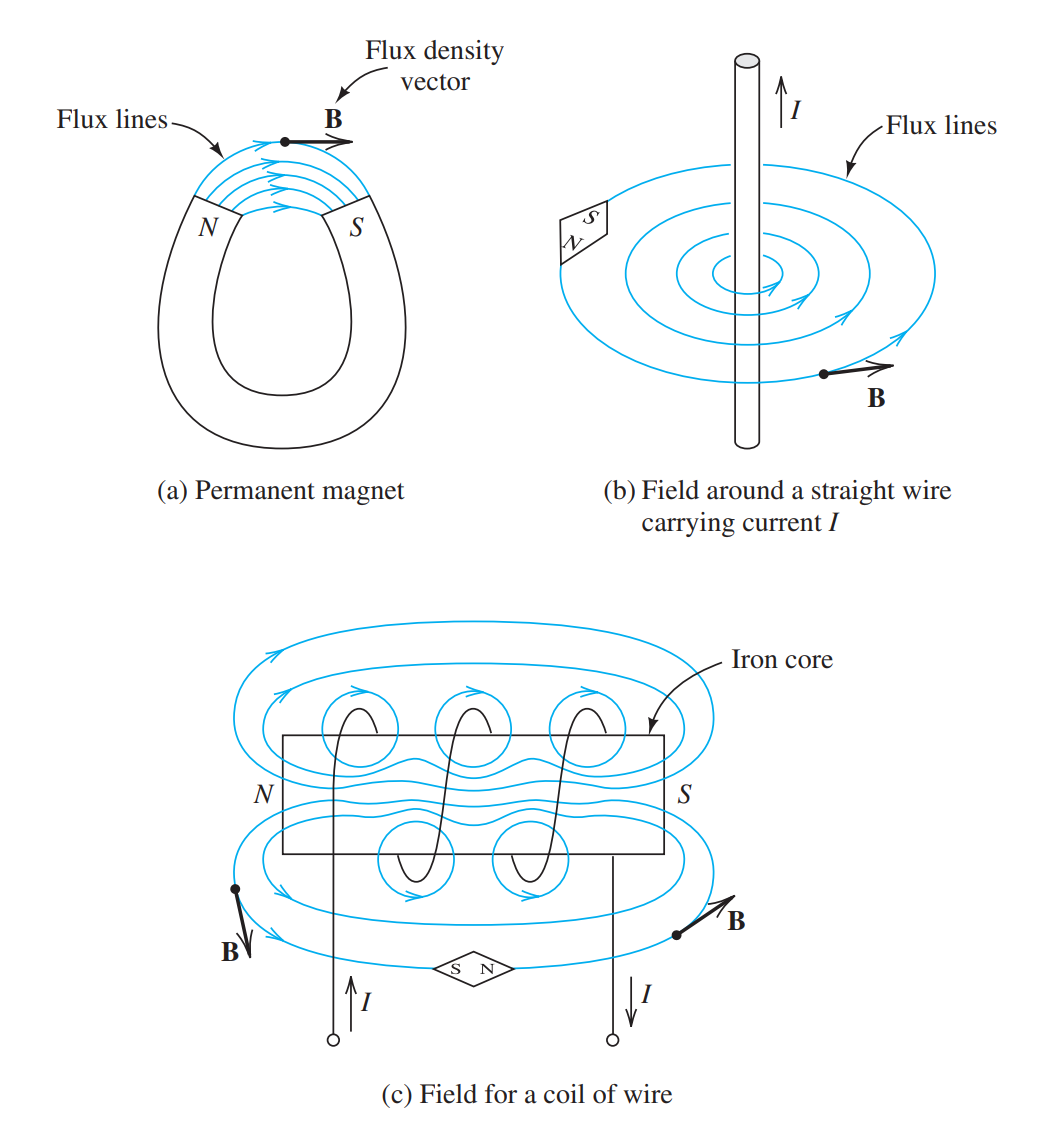
\includegraphics[width=0.4\linewidth]{images/magnetic-fields-lines.png}
    \caption{Magnetic fields can be visualized as lines of flux that form closed paths. Using a compass, we can determine the direction of the flux lines at any point. Note that the flux density vector $\symbfit{B}$ is tangent to the lines of flux.}
    \label{fig:magnetic-fields-lines}
\end{figure}
The units of magnetic field are webers. ($Wb$)
\begin{notebox}
    \begin{remark}
        Note that Flux lines leave the north-seeking end of a magnet and enter the south-seeking end.
    \end{remark}
\end{notebox}
\subsubsection{Magnetic Flux Density}
In equations, we represent the \textbf{magnetic flux density} as the vector quantity $\symbfit{B}$ and its corresponding lightface italic symbol $\textit{B}$ as the magnitude of the vector $\symbfit{B}$. The units of $\symbfit{B}$ are $webers/{meter}^2$ ($Wb/m^2$) or, equivalently, teslas ($\symbfit{T}$). The flux density vector $\symbfit{B}$ has a direction tangent to flux lines, as illustrated in Figure \ref{fig:magnetic-fields-lines}.
\subsection{Right-Hand Rule (Magnetic Field Direction)}
The direction of the magnetic field produced by a current can be determined by the right-hand rule. There are two interpretations of this rule.
\begin{enumerate}
    \item As illustrated in Figure \ref{fig:right-hand-rule-1}, if a wire is grasped with the thumb pointing in the direction of the current, the fingers encircle the wire, pointing in the direction of the magnetic field.
    \begin{figure}[H]
        \centering
        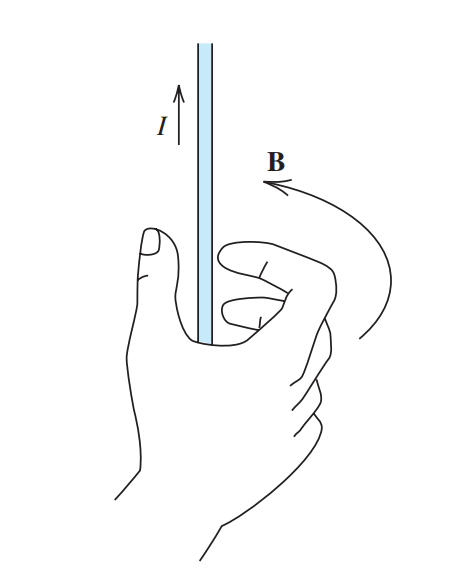
\includegraphics[width=0.3\linewidth]{images/right-hand-rule-1.png}
        \caption{Illustration 1}
        \label{fig:right-hand-rule-1}
    \end{figure}
    \item Moreover, as illustrated in \ref{fig:right-hand-rule-2}, if the fingers are wrapped around a coil in the direction of current flow, the thumb points in the direction of the magnetic field that is produced inside the coil.
    \begin{figure}[H]
        \centering
        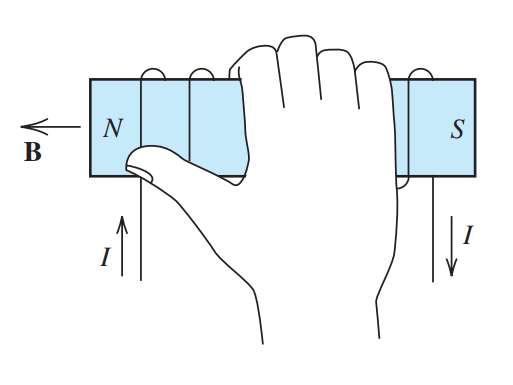
\includegraphics[width=0.3\linewidth]{images/right-hand-rule-2.png}
        \caption{Illustration 2}
        \label{fig:right-hand-rule-2}
    \end{figure}
\end{enumerate}
\begin{notebox}
    \begin{remark}
        The \textbf{direction of the magnetic field} is the {\color{red} \textbf{same}} as the \textbf{direction of the magnetic flux density}.
    \end{remark}
\end{notebox}
\subsection{Forces on Charges Moving in Magnetic Fields}
An electrical charge $q$ moving with velocity vector $\symbfit{u}$ through a magnetic field $\symbfit{B}$ experiences a force $\symbfit{f}$ as illustrated in Figure \ref{fig:forces-on-moving-charges-in-magnetic-fields}. The force vector is given by,
\begin{equation} \label{eq: force-vector}
    \symbfit{f} = q\symbfit{u} \times \symbfit{B}
\end{equation}
in which $\times$ represents the cross product. Because of the definition of cross product, we can know the magnitude of the force is given by
\begin{equation} \label{eq: force-vector-magnitude}
    f=quB~sin(\theta)
\end{equation}
in which, $\theta$ is the angle between $\symbfit{u}$ and $\symbfit{B}$, as illustrated in the figure \ref{fig:forces-on-moving-charges-in-magnetic-fields}.
\begin{figure}[H]
    \centering
    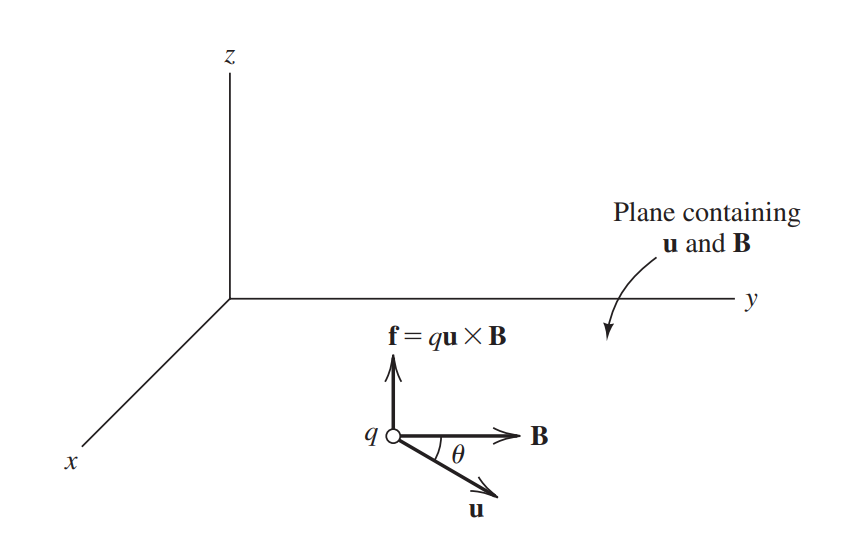
\includegraphics[width=0.5\linewidth]{images/forces-on-moving-charges-in-magnetic-fields.png}
    \caption{Forces on charges moving in magnetic fields}
    \label{fig:forces-on-moving-charges-in-magnetic-fields}
\end{figure}
\begin{notebox}
    \begin{remark}
    Note that
    \begin{enumerate}
        \item Force is exerted on a charge as it moves through a magnetic field.
        \item In the force vector equation \eqref{eq: force-vector}, the charge $q$ can be negative, which will opposite the direction of the force vector.
        \item In the magnitude of force vector equation \eqref{eq: force-vector-magnitude}, we always treat the charge $q$ to have no signs because magnitude is always a positive value.
    \end{enumerate}
    \end{remark}
\end{notebox}
\subsection{Forces on Current-Carrying Wires}
Force is exerted on a current-carrying conductor when it is immersed in a magnetic field. And the force is given by,
\begin{equation}
    d\symbfit{f} = id\symbfit{I} \times \symbfit{B} ~(?)
\end{equation}
in which the direction of $d\symbfit{I}$ and the reference direction for the current are the same. \newline
For a straight wire of length $l$ and a constant magnetic field, we have
\begin{equation}
    f=ilB~sin(\theta)
\end{equation}
in which $\theta$ is the angle between the wire and the field.
\begin{notebox}
    \begin{remark}
        Note that the force is maximized if the direction of the field is perpendicular to the wire because now $\theta=90\degree$, so $sin(\theta)=1$, thus $\symbfit{f}$ is maximized.
    \end{remark}
\end{notebox}
\subsection{Flux Linkages and Faraday's Law}
The magnetic flux passing through a surface area $\symbfit{A}$ is given by the surface integral
\begin{equation} \label{eq:magnetic-flux-general}
    \phi = \int_A\symbfit{B}\cdot d\symbfit{A}
\end{equation}
in which $d\symbfit{A}$ is an increment of area on the surface. The direction of the vector $d\symbfit{A}$ is perpendicular to the surface. If the magnetic flux density is constant and perpendicular to the surface, equation \eqref{eq:magnetic-flux-general} reduces to
\begin{equation}
    \phi = BA
\end{equation}
\begin{notebox}
    \begin{remark}
        We say $\phi$ is the magnetic flux or flux linking the coil but it is \textbf{not the flux linkages}.
    \end{remark}
\end{notebox}
We say that the flux passing through the surface bounded by a coil \textbf{links} the coil. If the coil has $\symbfit{N}$ turns, then the total {\color{red} \textbf{flux linkages}} are given by,
\begin{equation}
    \lambda =N\phi
\end{equation}
\begin{notebox}
    \begin{remark}
        Note that we say $\lambda$ is the {\color{red} \textbf{flux linkages}}, which will be useful in Faraday's law of magnetic induction.
    \end{remark}
\end{notebox}
According to {\color{red} \textbf{Faraday's law of magnetic induction}}, a {\color{red} \textbf{voltage}}
\begin{equation}
    e=\frac{d\lambda}{dt}
\end{equation}
is induced in coil whenever its \textbf{flux linkages} are changing. This can occur either because
\begin{enumerate}
    \item either the magnetic field is changing with time
    \item or because the coil is moving relative to a magnetic field.
\end{enumerate}
There are \textbf{two} ways to judge the \textbf{polarity of the induced voltage} or the \textbf{direction of the induced current}.
\subsubsection{Lenz's law}
\begin{thmbox}{Lenz's Law}{lenz-law}
    The \textbf{Lenz's law} states that the polarity of the induced voltage is such that the voltage would produce a current (through an external resistance) that \textbf{opposes} the original change in flux linkages.
\end{thmbox}
\subsubsection{Right-Hand Rule}
This rule only applies when the voltage is induced in a conductor moving through a magnetic field.
\subsection{Voltages Induced in Field-Cutting Conductors}
For example, considering Figure \ref{fig:voltage-induced-in-field-cutting-conductors}. A uniform magnetic field is directed into the page. The sliding conductor and the stationary rails form a loop having an area of $A=lx$. The flux linkages of the coil are
\begin{displaymath}
    \lambda = BA = Blx
\end{displaymath}
According to Faraday's law, the voltage induced in the coil is given by
\begin{displaymath}
    e=\frac{d\lambda}{dt}=Bl\frac{dx}{dt}
\end{displaymath}
However, $u=dx/dt$ is the velocity of the sliding conductor, so we have
\begin{equation}
    e=Blu
\end{equation}
\begin{figure}[H]
    \centering
    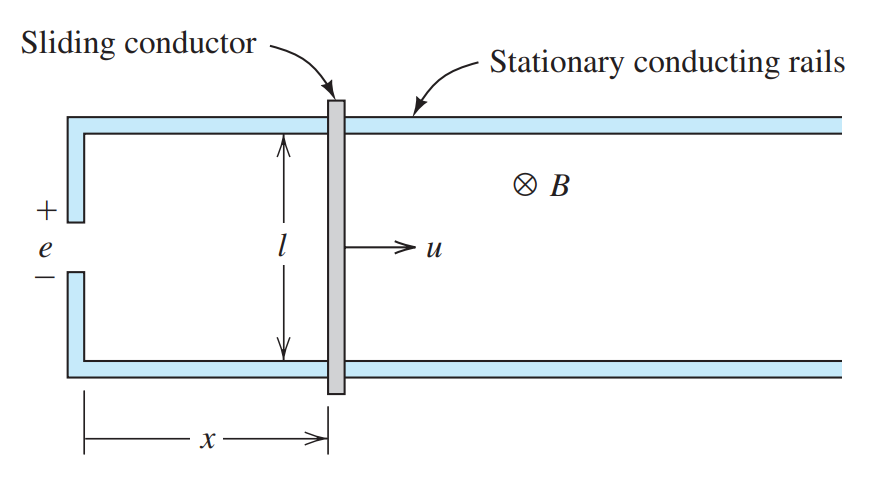
\includegraphics[width=0.5\linewidth]{images/voltage-induced-in-field-cutting-conductors.png}
    \caption{Voltage Induced in Field-Cutting Conductors}
    \label{fig:voltage-induced-in-field-cutting-conductors}
\end{figure}
\begin{notebox}
    \begin{remark}
        The general solution to the induced voltage $\symbfit{e}$ is to use {\color{red} \textbf{Faraday's law of magnetic induction}}.
    \end{remark}
\end{notebox}
\section{Inductance and Mutual Inductance}
We have seen that when a coil carries current, a magnetic flux is produced that links the coil. If the current changes with time, the flux also changes, inducing a voltage in the coil. This is the physical basis of inductance. \newline
Consider a coil carrying a current $i$ that sets up a flux $\phi$ linking the coil. The inductance of the coil can be defined as flux linkages divided by current:
\begin{equation} \label{eq:definition-of-inductance}
    L=\frac{\lambda}{i}
\end{equation}
Assuming that the flux is confined to the core that all of the flux links all of the turns, we care write $\lambda =N\phi$. Then, we have
\begin{equation}
    L=\frac{N\phi}{i}
\end{equation}
According to Faraday's law, voltage is induced in a coil when its flux linkages change:
\begin{displaymath}
    e=\frac{d\lambda}{dt}
\end{displaymath}
Rearranging the equation \eqref{eq:definition-of-inductance}, we have $\lambda = Li$. Substituting this for $\lambda$ in the Faraday's law, we get
\begin{equation}
    e=\frac{d(Li)}{dt}
\end{equation}
For a coil wound on a stationary core, the inductance is constant with time, and the above equation reduces to
\begin{equation}
    e=L\frac{di}{dt}
\end{equation}
Of course, this is the equation relating voltage and current that we used to analyze circuits containing inductance.
\subsection{Mutual Inductance}
\section{Ideal Transformers}
A transformer consists of several coils wound on a common core that usually consists of laminated iron (to reduce eddy-current loss). We will see that transformers can be used to adjust the values of ac voltages. Transformers can greatly facilitate power distribution by stepping voltage up (2400$V$ can be stepped up to 48$kV$) and down (2400$V$ can be stepped down to $240V$) at various points in the distribution system.
\subsection{Voltage Ratio}
A transformer is illustrated in Figure \ref{fig:transformer}. An ac voltage source is connected to the primary coil, which consists of $N_1$ turns of wire. Current flows into the primary side and causes an ac magnetic flux $\phi (t)$ to appear in the core. This flux induces a voltage \textbf{of the same frequency} in the $N_2$-turn secondary coil, which delivers power to the load. However, the voltage will be different according to the number of loops in each coil.
\begin{figure}[H]
    \centering
    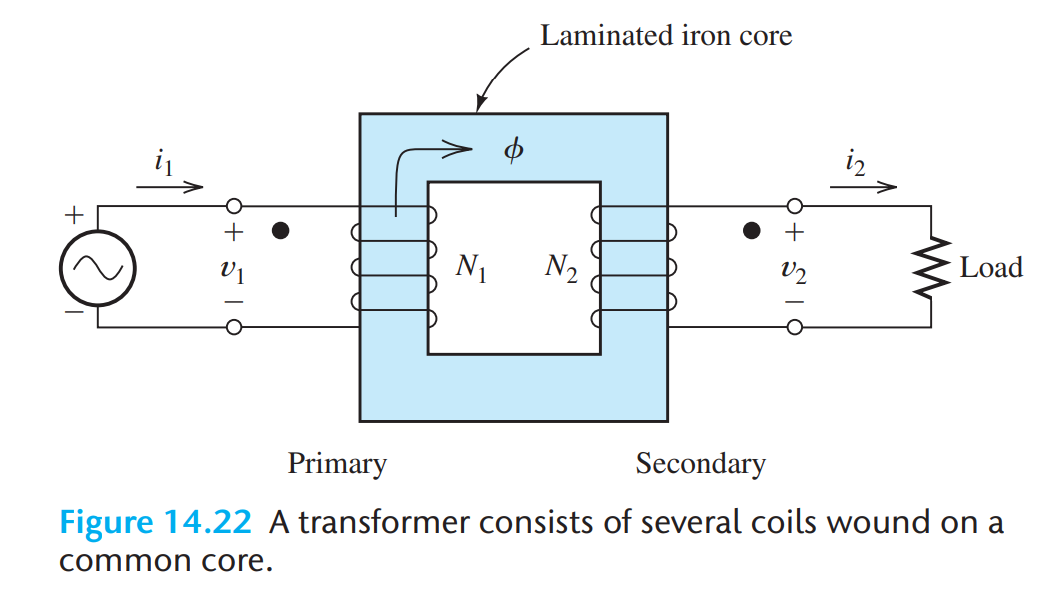
\includegraphics[width=0.5\linewidth]{images/transformer.png}
    \caption{Transformer}
    \label{fig:transformer}
\end{figure}
From Faraday's Law, the voltage or emf induced in the secondary coil is
\begin{equation}
    V_2=N_2\frac{d\phi_B}{dt}
\end{equation}
where $N_2$ is the number of turns in the secondary coil, and $d\phi_B/dt$ is the rate at which the magnetic flux changes. \newline
The input primary voltage, $V_1$, is related to the rate at which the flux changes through it,
\begin{equation}
    V_1=N_1\frac{d\phi_B}{dt}
\end{equation}
where $N_1$ is the number of turns in the primary coil. This follows because the changing flux produces a back emf, $N_1d\phi_B/dt$ that exactly balances the applied voltage $V_1$ if the resistance of the primary can be ignored (Kirchhoff's rules). We divide these two equations, assuming little or no flux is lost, to find
\begin{equation} \label{eq:voltage-ratio-transformer}
    \frac{V_1}{V_2} = \frac{N_1}{N_2}
\end{equation}
This \textbf{transformer equation} \eqref{eq:voltage-ratio-transformer} tells how the secondary (output) voltage is related to the primary (input) voltage; $V_1$ and $V_2$ in equation \eqref{eq:voltage-ratio-transformer} can be the \textbf{rms} values for both, or peak values for both.
\begin{notebox}
    \begin{remark}
        DC voltages don't work in a transformer because there would be no changing magnetic flux.
    \end{remark}
\end{notebox}
\subsection{Current Ratio}
Although ac voltage can be increased (or decreased) with a transformer, we don't get something for nothing. Energy conservation tells us that the  \textbf{power output can be no greater than the power input}. A well-designed transformer can be greater than 99\% efficient, so little energy is lost to heat. The power output thus essentially equals the power input. Since power $P=IV$, we have
\begin{equation}
    I_1V_1=I_2=V_2
\end{equation}
or
\begin{equation} \label{eq:current-ratio-transformer}
    \frac{I_1}{I_2} = \frac{N_2}{N_1}
\end{equation}
\end{document}
